\documentclass[english]{report}


\setlength {\marginparwidth }{2cm} 
\usepackage{todonotes}

\usepackage[perpage,para,symbol]{footmisc}

\hyphenpenalty=15000 
\tolerance=1000

\usepackage{tikz}
\usetikzlibrary{arrows,decorations.pathmorphing,backgrounds,fit,positioning,calc,shapes}
\usepackage{pgfmath}
\usepackage{pgfplots}
\usepgfplotslibrary{external} 
\tikzexternalize
\usepackage{rotating}
\usepackage{array}	
\usepackage{graphicx}
\usepackage{float}	
\usepackage{mdwlist}
\usepackage{setspace}
\usepackage{listings}
\usepackage{bytefield}
\usepackage{tabularx}
\usepackage{multirow}	       
\usepackage{caption} 
\captionsetup[table]{skip=10pt}

\usepackage{url}               
\usepackage{hyperref}
\usepackage[all]{hypcap}	
\usepackage{titlesec}
\setcounter{secnumdepth}{4}
\titleformat{\paragraph}
{\normalfont\normalsize\bfseries}{\theparagraph}{1em}{}
\titlespacing*{\paragraph}
{0pt}{3.25ex plus 1ex minus .2ex}{1.5ex plus .2ex}
\hypersetup{colorlinks,breaklinks,
            linkcolor=darkblue,urlcolor=darkblue,
            anchorcolor=darkblue,citecolor=darkblue}


\definecolor{darkblue}{rgb}{0.0,0.0,0.3} 
\definecolor{darkred}{rgb}{0.4,0.0,0.0}
\definecolor{red}{rgb}{0.7,0.0,0.0}
\definecolor{lightgrey}{rgb}{0.8,0.8,0.8} 
\definecolor{grey}{rgb}{0.6,0.6,0.6}
\definecolor{darkgrey}{rgb}{0.4,0.4,0.4}
\definecolor{aqua}{rgb}{0.0, 1.0, 1.0}
\definecolor{dkgreen}{rgb}{0,0.6,0}
\definecolor{gray}{rgb}{0.5,0.5,0.5}
\definecolor{mauve}{rgb}{0.58,0,0.82}

\lstset{
  language=C,
  showstringspaces=false,
  columns=flexible,
  basicstyle={\small\ttfamily},
  numbers=none,
  numberstyle=\tiny\color{gray},
  keywordstyle=\color{blue},
  commentstyle=\color{dkgreen},
  stringstyle=\color{mauve},
  breaklines=true,
  breakatwhitespace=true,
  tabsize=3
}
\usepackage{listings}
\PassOptionsToPackage{USenglish,english}{babel} 
\usepackage{csquotes}
\usepackage[USenglish,english]{babel}
\usepackage[acronym, section=section, nonumberlist, nomain, nopostdot]{glossaries}
\makeglossaries
 
\makeglossaries
\newcommand{\colorbitbox}[3]{%
	\rlap{\bitbox{#2}{\color{#1}\rule{\width}{\height}}}%
	\bitbox{#2}{#3}}

\renewcommand{\thesubsection}{\alph{subsection}}

\begin{document}

\title{Homework 3}
\author{Calin Capitanu}

\maketitle

\clearpage
\chapter{Two Research Studies}
\section{Code Comments}

\subsection{Can we draw the conclusion that comments improve the code? Explain}

In my opinion, there is no good conclusion that can be drawn in a generalized form from a simple experiment like this. This is mostly because the dataset of the experiment is too little, and the conclusions drawn from it are too generalized. \\
Besides the term ``best'' being hardly described, and considered not relevant for this, which in my opinion, is wrong, as intuition could lead to ``best'' meaning performance in speed and capacity, which comments are unrelated to, but to the process of development, they could be. This is extrapolating the different known and unknown parts of the problem, but the main idea is that there can be no hard conclusions being drawn after such a small experiment, with only 2 data points.

\subsection{Suggest improvements to the study!}

As the previous part suggests, that the wrong part here in my opinion is the size of the dataset. In this case, I think the best way of improving the experiment and the conclusions from it are to increase the size of the sample data, as well as to formulate the conclusion as if was part of an experiment and that the probability of a program being ``better'' is when it has comments.\\
Moreover, I think that defining the ``best'' term for a program is crucial, as one can also better describe which program is better with more scientific proof and less statistical results.

\clearpage

\section{Functional Programming}

\subsection{Can we draw the conclusion that functional programming languages give slower code? Explain!}

Similar to the previous example, in my opinion, the problem space is too large, while the input data set is too little in this programming language example. That is, only one problem has been tested, only one functional programming language has been tested and also that only one solution to the problem is taken into account. With this little amound of information, there is no way we can draw definite conclusions to such generalized statements such as ``functional programming languages being slower''. At the same time, the fact that two different teams were assigned to this experiments also means that the solution conceptually could highly differ.

\subsection{Suggest improvements to the study!}

In order to improve this experiment, I think that the best way is to define a smaller sample space of the problem, thus first things first trying to define a smaller goal conclusion. In order tu study if the wanted conclusion holds, we need to take into account less variables unrelated to the problem (such as different solutions from different teams).\\
First things first, I suggest that the same team, with the same conceptual solution codes the same problem into the two different programming languages.\\
Secondly, I suggest that the conclusion data is restricted only to Haskell, and not to functional programming languages in general, since they could differ a lot.
Finally, I think that the best way to rephrase the conclusion is to add some sort of statistical or probability factor. That is, even if after all the previous points, Haskell still yield slower times than Java for this specific problem and some others, there could be some other problem in which the result is the opposite, thus bringing the uncertainty factor of the term ``on average'', the conclusion could be more feasible.

\chapter{Zipf's law}

\subsection{Dataset}

The dataset that I chose is the frequency of words in English, since the format offered allows for easy reading into a programming language of choice and proper formatting and analysis from that point.

\subsection{Graph}

The graph below (Figure 2.1) represents the plot of English word frequency plotted against the rank of their appearance in a log-log plot.

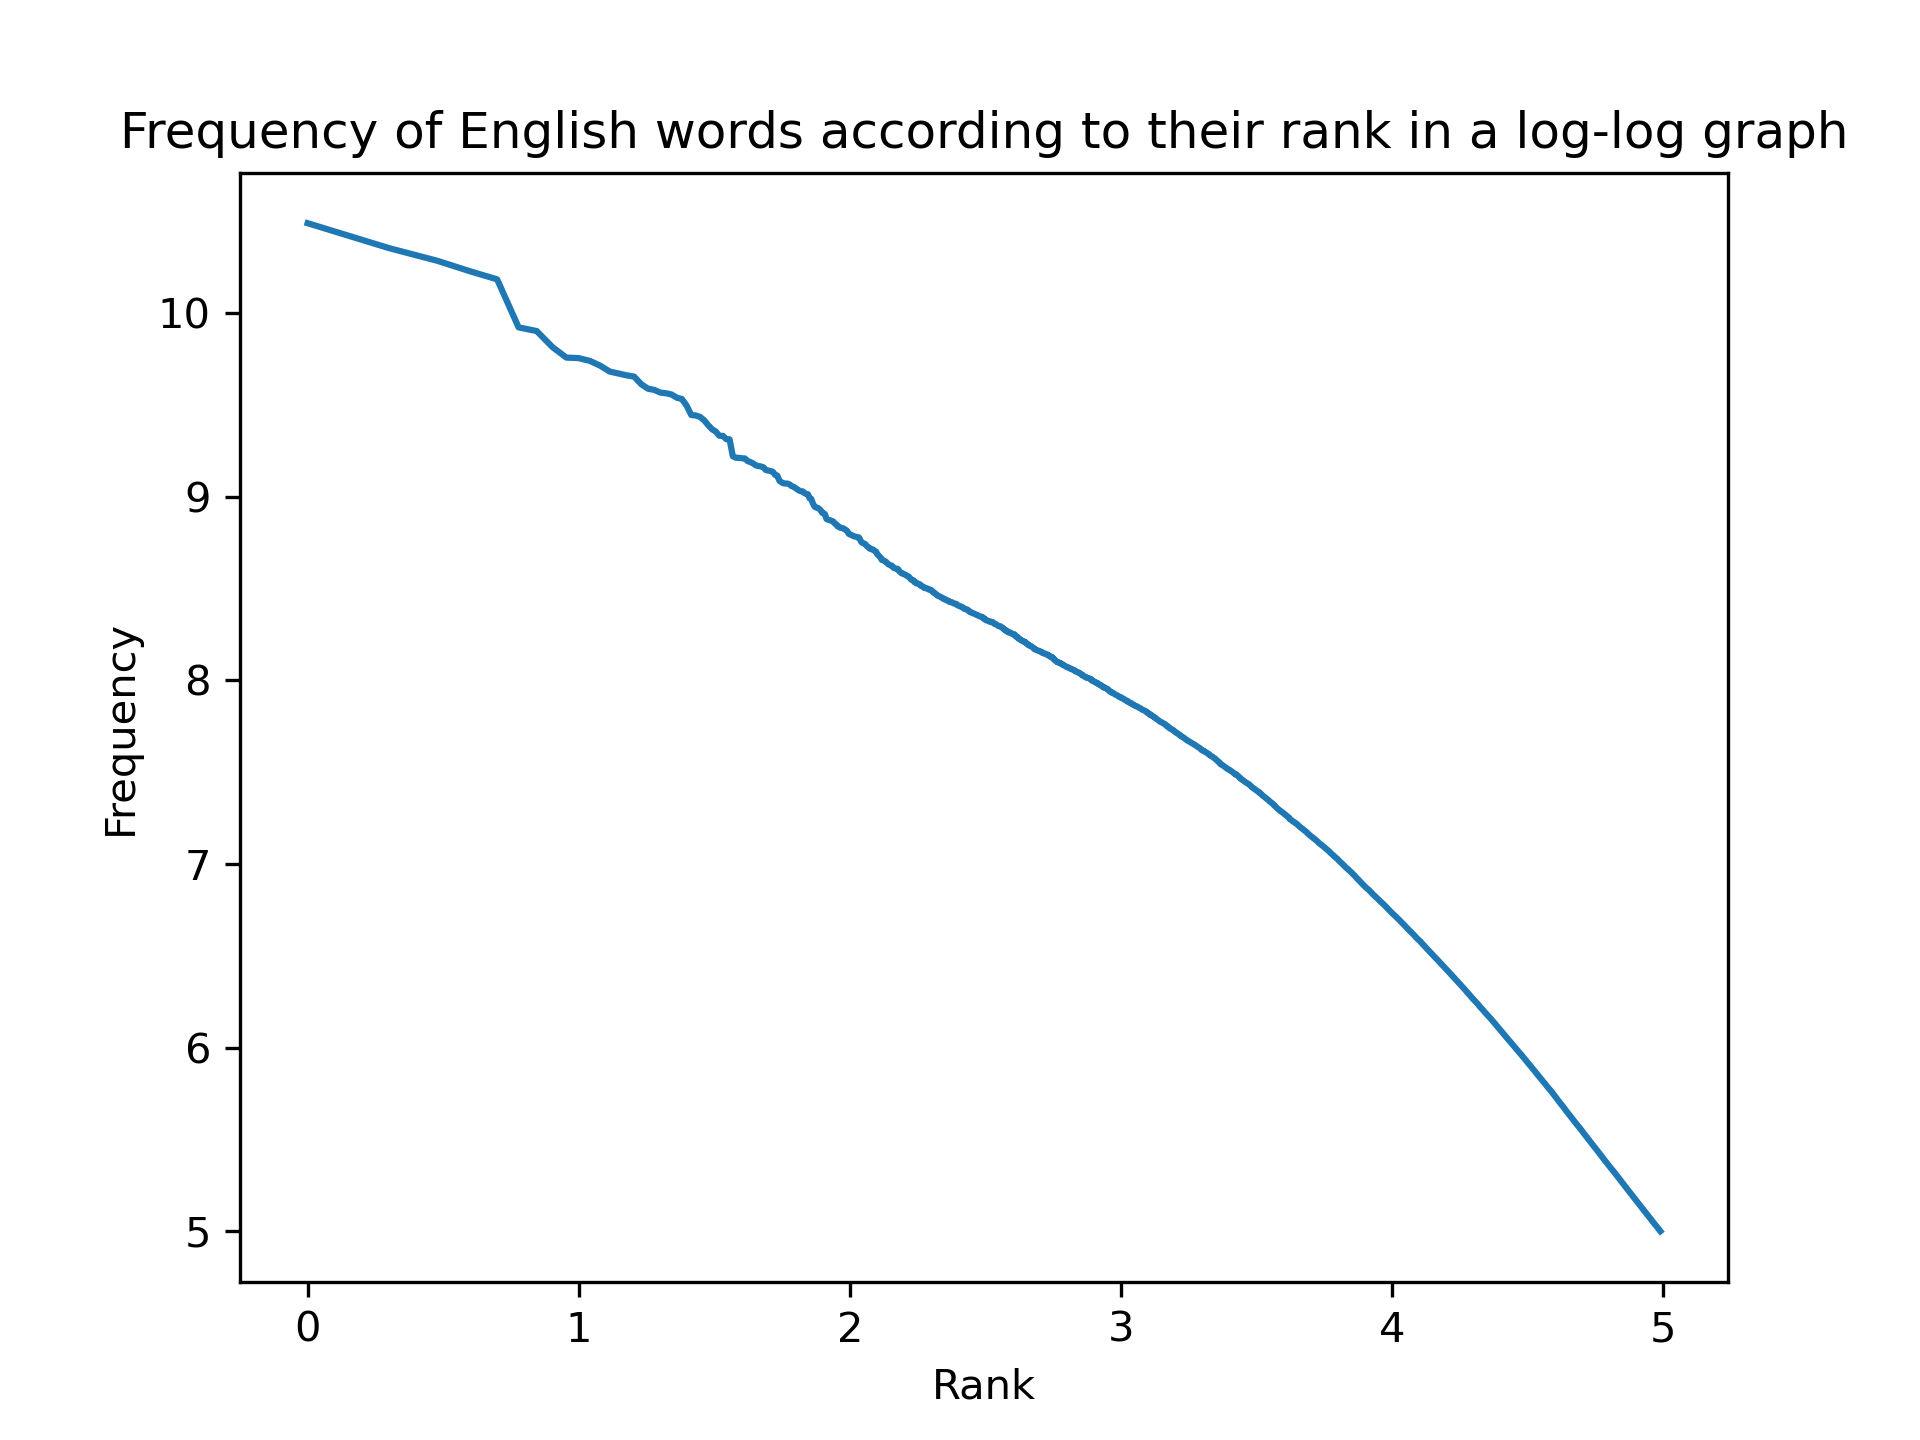
\includegraphics[scale=0.65]{histogram.png}

\subsection{Linear Regression}

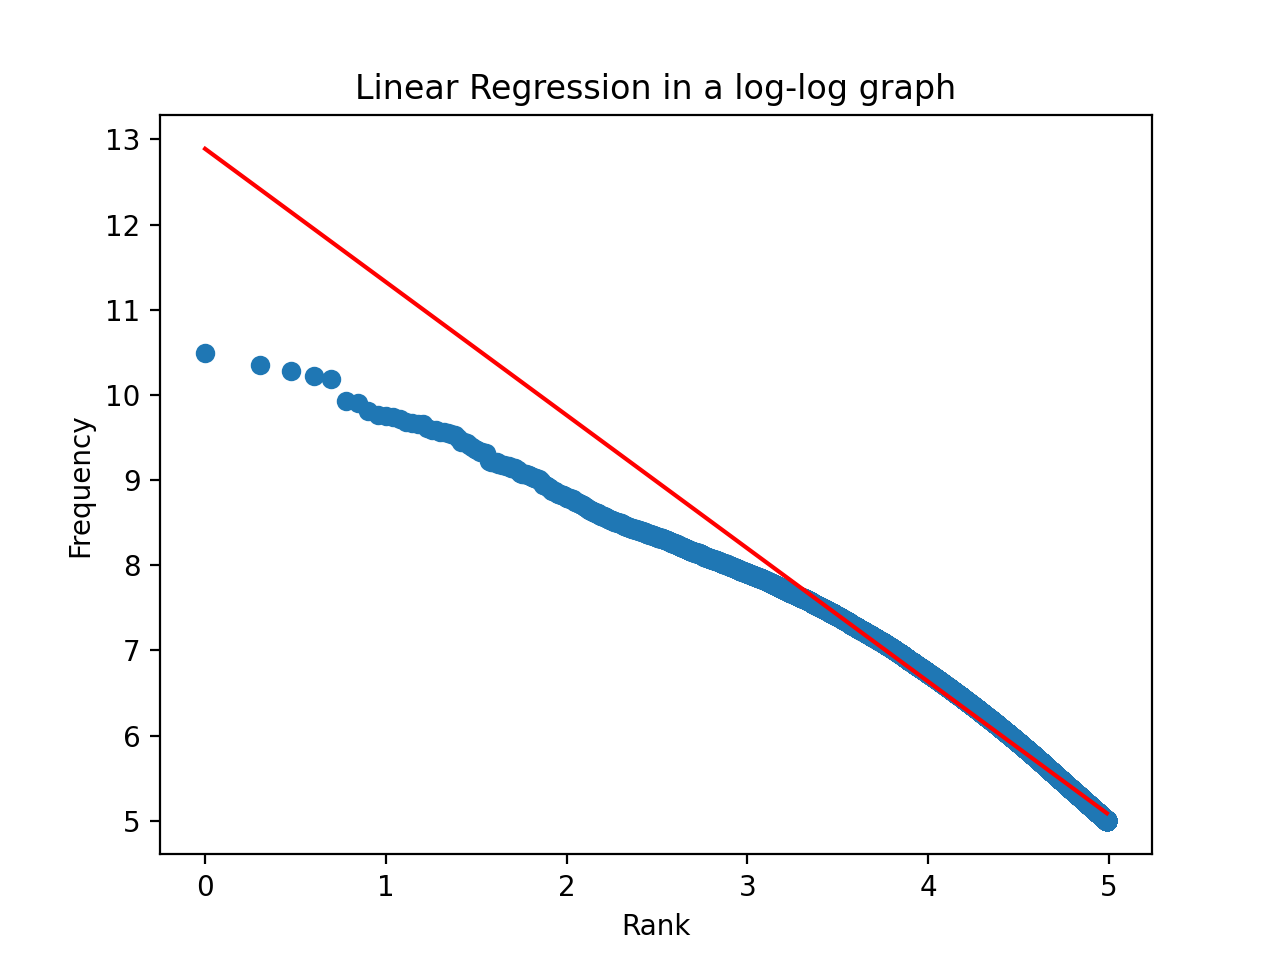
\includegraphics[scale=0.65]{lr.png}

The results here show a pretty well fit in the latter part of the graph. Function's coefficient sits around -1.563, since I inputted the points already under the log function. But then, since we want the un-logged coefficient, I will get 0.027307183730692054.
\\
If we take the linearly fitted line, the data holds with Zipf's law.

\subsection{Scientific Article}

In the scientific article ``Zipf’s Law for Word Frequencies: Word Forms versus Lemmas in Long Texts'', teh results shown are a bit different than the one here.\\
To start with, the graphs are relatively similar under the log function, but the coefficient resulted in my research is a bit below 10 times smaller than the cited paper. \cite{zipf}

\subsection{Scientific Statement}

In my opinion, I think that Zipf's Law is a conjecture. A conjecture is an opinion or a conclusion formed on the basis of inclomplete information. That is, this is not a theory that can always hold, since you do need to find a linear fit in order to make it ``more true''. In this case, this is just some sort of approximation of observable data, in which case, I think it is a conjecture.

\bibliographystyle{myIEEEtran}
\renewcommand{\bibname}{References}
\addcontentsline{toc}{chapter}{References}
\bibliography{references}

\end{document}
